% SNT - 2019
% (C) Stéphane Colomban (CC : sd-by-sa)




\documentclass[a4paper,10pt]{article}
\usepackage[rgb]{xcolor}
\usepackage[utf8]{inputenc}
\usepackage[T1]{fontenc}
\usepackage[frenchb]{babel}
\usepackage{mathrsfs, amsmath, amssymb}
\usepackage{times,mathptmx}
\DeclareSymbolFont{lmodern}{U}{euex}{m}{n}
\DeclareMathSymbol\infty \mathord{lmodern}{"31}
\usepackage[scaled=0.875]{helvet} % ss
\usepackage{textcomp}
\usepackage{dsfont} % pour les symboles des ensembles
\usepackage[left=2cm,right=2cm,top=0.5cm,bottom=2cm]{geometry}
\usepackage{fancyhdr} 
\fancyhf{}
\setlength{\headheight}{26pt}
\setlength{\footskip}{18pt}
\renewcommand {\headrulewidth}{0pt}
\renewcommand {\footrulewidth}{1pt}

\usepackage{hyperxmp}
\usepackage{listings}
%\usepackage[colorlinks=true,pdfstartview=FitV,linkcolor=blue,citecolor=blue,urlcolor=blue]{hyperref}
\pagestyle{fancy}
\usepackage {array}
\usepackage{tabularx}
\usepackage{multirow}
\usepackage{fltpoint}
\usepackage{pstricks,pst-all,pstricks-add,pst-tree,pst-3dplot,pst-func}
\usepackage{ifthen}
\usepackage{calc}
\usepackage{esvect}
\usepackage[np]{numprint}
\usepackage{pgf}
\usepackage{mathrsfs}
\usepackage{tikz}
\usetikzlibrary{arrows}
\usetikzlibrary[patterns]
\usetikzlibrary{shapes.misc}
\usetikzlibrary{decorations.pathmorphing,calc,shapes,shapes.geometric,patterns}
\setlength{\parindent}{0mm}
\usepackage [alwaysadjust]{paralist}
\usepackage{times,tcolorbox}
\usepackage{luatex85}
\usepackage{listings}
\usepackage{hyperref}
\hypersetup{
    colorlinks=true,
    linkcolor=blue,
    filecolor=magenta,      
    urlcolor=blue
}
    
    
\setdefaultenum {1.}{a)}{}{}
\hyphenpenalty 10000 
\renewcommand*{\tabularxcolumn}[1]{m{#1}} 
\newcommand{\Oij}{$\left( {{\mathrm{O}};\vec i,\vec j} \right)$}
\newcommand{\Oijk}{$\left( {{\mathrm{O}};\vec i,\vec j ,\vec k} \right)$}
\newcommand{\euro}{\texteuro{}}
\newcommand{\R}{\mathds {R}}
\newcommand{\N}{\mathds {N}}
\newcommand{\Z}{\mathds {Z}}
\newcommand{\Q}{\mathds {Q}}
\newcommand{\e}{\mathrm {e}}
\newcommand{\dd}{\,\mathrm{d}}

\newcommand\pts[1][]{ \textcolor{red} { \hfill #1 pts}} 
\newcommand\pt[1][]{ \textcolor{red} { \hfill #1 pt}} 

\DecimalMathComma
\definecolor{jaune}{rgb} {0.9529,0.9215,0.04705}
\definecolor{bleu}{rgb} {0,0.3725,0.698}
\definecolor{rouge}{rgb} {0.9294,0.1529,0.1411} 
\definecolor{bleuvif}{rgb} {0.01569,0.12941,0.25098}
\definecolor{orange}{rgb} {.9,0.4216,0.06} 
\definecolor{bleuclair}{rgb} {0.2,0.9,1}
\definecolor{vertclair}{rgb} {0.9,1,.8}
\definecolor{vert}{rgb} {0.1,0.6,0.1}
%%%%%%%%%%%%%%%%%%%%%%%%%%%%%%%%%%%%%%%%%%%%%%%%%%%%%%%%%%%%%%%%%%%%%%%%%%%%%%
\newcommand \SNT[3]{

\begin{minipage}{3cm}
\begin{flushleft}
\begin{tikzpicture}[line cap=round,line join=round,>=triangle 45,x=.5cm,y=.5cm]

\draw [color=black, fill=white]  (0.,0.) rectangle (7,5) ;
\draw [color=black, fill=bleuclair]  (0.0,3.5) rectangle (7,5) ;

\draw [color=black] (3.5,3.5) node[above] {\textbf{{\Large SNT -- ELLA }}};
\draw [color=bleuvif] (3.5,2) node[above] { \textbf{\textsc{#1}}};
\draw [color=bleuvif] (3.5,1) node[above] { \textbf{\textsc{#2}}};
\end{tikzpicture}
\end{flushleft}
\end{minipage}
\begin{minipage}{15cm}

  \begin{center} 
   
  \textbf{\textcolor{black}{{\textsc{\Large #3 }}}}\\ 

  \end{center}
\end{minipage}

  
  }


%%%%%%%%%%%%%%%%%%%%%%%%%%%%%%%%%%%%%%%%%%%%%%%%%%%%%%%%%%%%%%%%%%%%%%%%%%%%%%  
\newtcbox{\boitearrondie}{colframe=black, colback=jaune, boxrule=1pt, arc=4pt,
  boxsep=2pt,left=10pt,right=10pt,top=10pt,bottom=10pt}



%%%%%%%%%%%%%%%%%%%%%%%%%%%%%%%%%%%%%%%%%%%%%%%%%%%%%%%%%%%%%%%%%%%%%%%%%%%%%%
\newcommand \remarque[3]{
     \begin{tikzpicture}[line cap=round,line join=round,>=triangle 45,x=.07cm,y=.07cm]
       
       \draw[color=red,ultra thick, fill=black] (11,0) node[anchor=west, scale=.8, right] {\Large \color{ #1!} \textsc{\textbf{#3}}};
     \draw[color=#1!110,ultra thick, fill=#1!75](0,0) circle (6);
        {\clip (0,0) circle (12);
       
		   
        \draw[color=white,ultra thick, fill=white] (0,0) node[scale=1] {\huge  \textbf{#2}};
        }
        
  \end{tikzpicture}
}

%%%%%%%%%%%%%%%%%%%%%%%%%%%%%%%%%%%%%%%%%%%%%%%%%%%%%%%%%%%%%%%%%%%%%%%%%%%%%%


%%%%%%%%%%%%%%%%%%%%%%%%%%%%%%%%%%%%%%%%%%%%%%%%%%%%%%%%%%%%%%%%%%%%%%%%%%%%%%
\newcommand\cadre[1]{
\boitearrondie{
\begin{minipage}{\textwidth-30pt}
#1
\end{minipage}
}
}

%%%%%%%%%%%%%%%%%%%%%%%%%%%%%%%%%%%%%%%%%%%%%%%%%%%%%%%%%%%%%%%%%%%%%%%%%%%%%% 
% Programme en Python
 
 
\lstset{
backgroundcolor=\color{vertclair},
frame=single,
rulecolor=\color{vert},
framexleftmargin=2em,
framexbottommargin=3pt,
frame=tb,
%keepspaces=t
language=Python,
numbersep=1em,
numberstyle      = \scriptsize\color{black},
numbersep        = 20pt,
framextopmargin=5pt,
framexbottommargin=5pt,
showspaces=false,
showtabs=false,
showstringspaces=false,
tabsize=4,
% Basic
basicstyle=\ttfamily\footnotesize\bfseries,
% Strings
stringstyle=\color{red}\bfseries,
morecomment=[s][\color{red}]{"""}{"""},
morecomment=[s][\color{red}]{'''}{'''},
%% keywords
keywordstyle={\textbf{\color{black}\bfseries}},
% additional keywords
keywordstyle={[2]\color{blue}},
commentstyle=\color{darkgray}\ttfamily,  extendedchars=true,
    literate=
    {á}{{\'a}}1 {é}{{\'e}}1 {í}{{\'i}}1 {ó}{{\'o}}1 {ú}{{\'u}}1
    {Á}{{\'A}}1 {É}{{\'E}}1 {Í}{{\'I}}1 {Ó}{{\'O}}1 {Ú}{{\'U}}1
    {à}{{\`a}}1 {è}{{\`e}}1 {ì}{{\`i}}1 {ò}{{\`o}}1 {ù}{{\`u}}1
    {À}{{\`A}}1 {È}{{\'E}}1 {Ì}{{\`I}}1 {Ò}{{\`O}}1 {Ù}{{\`U}}1
    {ä}{{\"a}}1 {ë}{{\"e}}1 {ï}{{\"i}}1 {ö}{{\"o}}1 {ü}{{\"u}}1
    {Ä}{{\"A}}1 {Ë}{{\"E}}1 {Ï}{{\"I}}1 {Ö}{{\"O}}1 {Ü}{{\"U}}1
    {â}{{\^a}}1 {ê}{{\^e}}1 {î}{{\^i}}1 {ô}{{\^o}}1 {û}{{\^u}}1
    {Â}{{\^A}}1 {Ê}{{\^E}}1 {Î}{{\^I}}1 {Ô}{{\^O}}1 {Û}{{\^U}}1
    {œ}{{\oe}}1 {Œ}{{\OE}}1 {æ}{{\ae}}1 {Æ}{{\AE}}1 {ß}{{\ss}}1
    {ç}{{\c c}}1 {Ç}{{\c C}}1 {ø}{{\o}}1 {å}{{\r a}}1 {Å}{{\r A}}1
    {€}{{\EUR}}1 {£}{{\pounds}}1
}




\lfoot{ \vspace{-0.5cm }\copyright \quad  S. COLOMBAN - 2019}
\rfoot{ 
\includegraphics[width=1.8cm]{by-nc-sa.eu.eps} }

\begin{document}

\SNT{Cartographie}{Géolocalisation}{Séance 1 - Introduction aux coordonnées GPS}

\bigskip


\begin{center}
{\large \textbf{Partie 1 : Principe du GPS et des coordonnées GPS }}
\hrulefill
\end{center}

\remarque{orange}{>}{Préambule}

Le Global Positioning System (GPS) ou « Géo-positionnement par satellite », est un système de positionnement par satellites appartenant au gouvernement des États-Unis. Mis en place par le département de la Défense des États-Unis à des fins militaires à partir de 1973, le système avec 24 satellites est totalement opérationnel en 1995 et s'ouvre au civil en 2000.
\begin{flushright}{\small source Wikipédia}\end{flushright}

\remarque{blue}{?}{Fonctionnement}

\begin{minipage}[]{.7\textwidth}

Les 24 satellites de constellation gps sont  situés à 20184 km d’altitude, et font  le tour de la terre en 12h. 
 

Le principe de fonctionnement du GPS repose sur la triangulation.

\medskip

Chaque satellite émet une onde électromagnétique de vitesse connue. Cette onde est émise à un temps bien déterminé. Le récepteur calcule ensuite le temps de transmission. En multipliant ce temps par la vitesse, il obtient donc la distance qui le sépare du satellite.

\medskip

Le récepteur effectue ce calcul sur un premier satellite et  dispose d’une première information : il se trouve sur une sphere centrée sur le satellite. 

En répétant cette procédure avec deux autres stallites , il peut à nouveau se situer sur deux autres sphères centrées  sur les deux satellites. 

En cherchant la zone d’intersection entre ces trois sphère, on obtient la position sur la Terre. 

\medskip
Un  quatrième satellite est necessaire afin d'affiner la position. Plus le nombre de satellites captés sera important, meilleure sera la précision.

L’extraordinaire précision des horloges atomiques est indispensable, car une erreur d’un millième de seconde dans le calcul du temps de transmission entrainerait une erreur de positionnement de 300 km !
\end{minipage}
\begin{minipage}[]{.3\textwidth}
\begin{flushright} 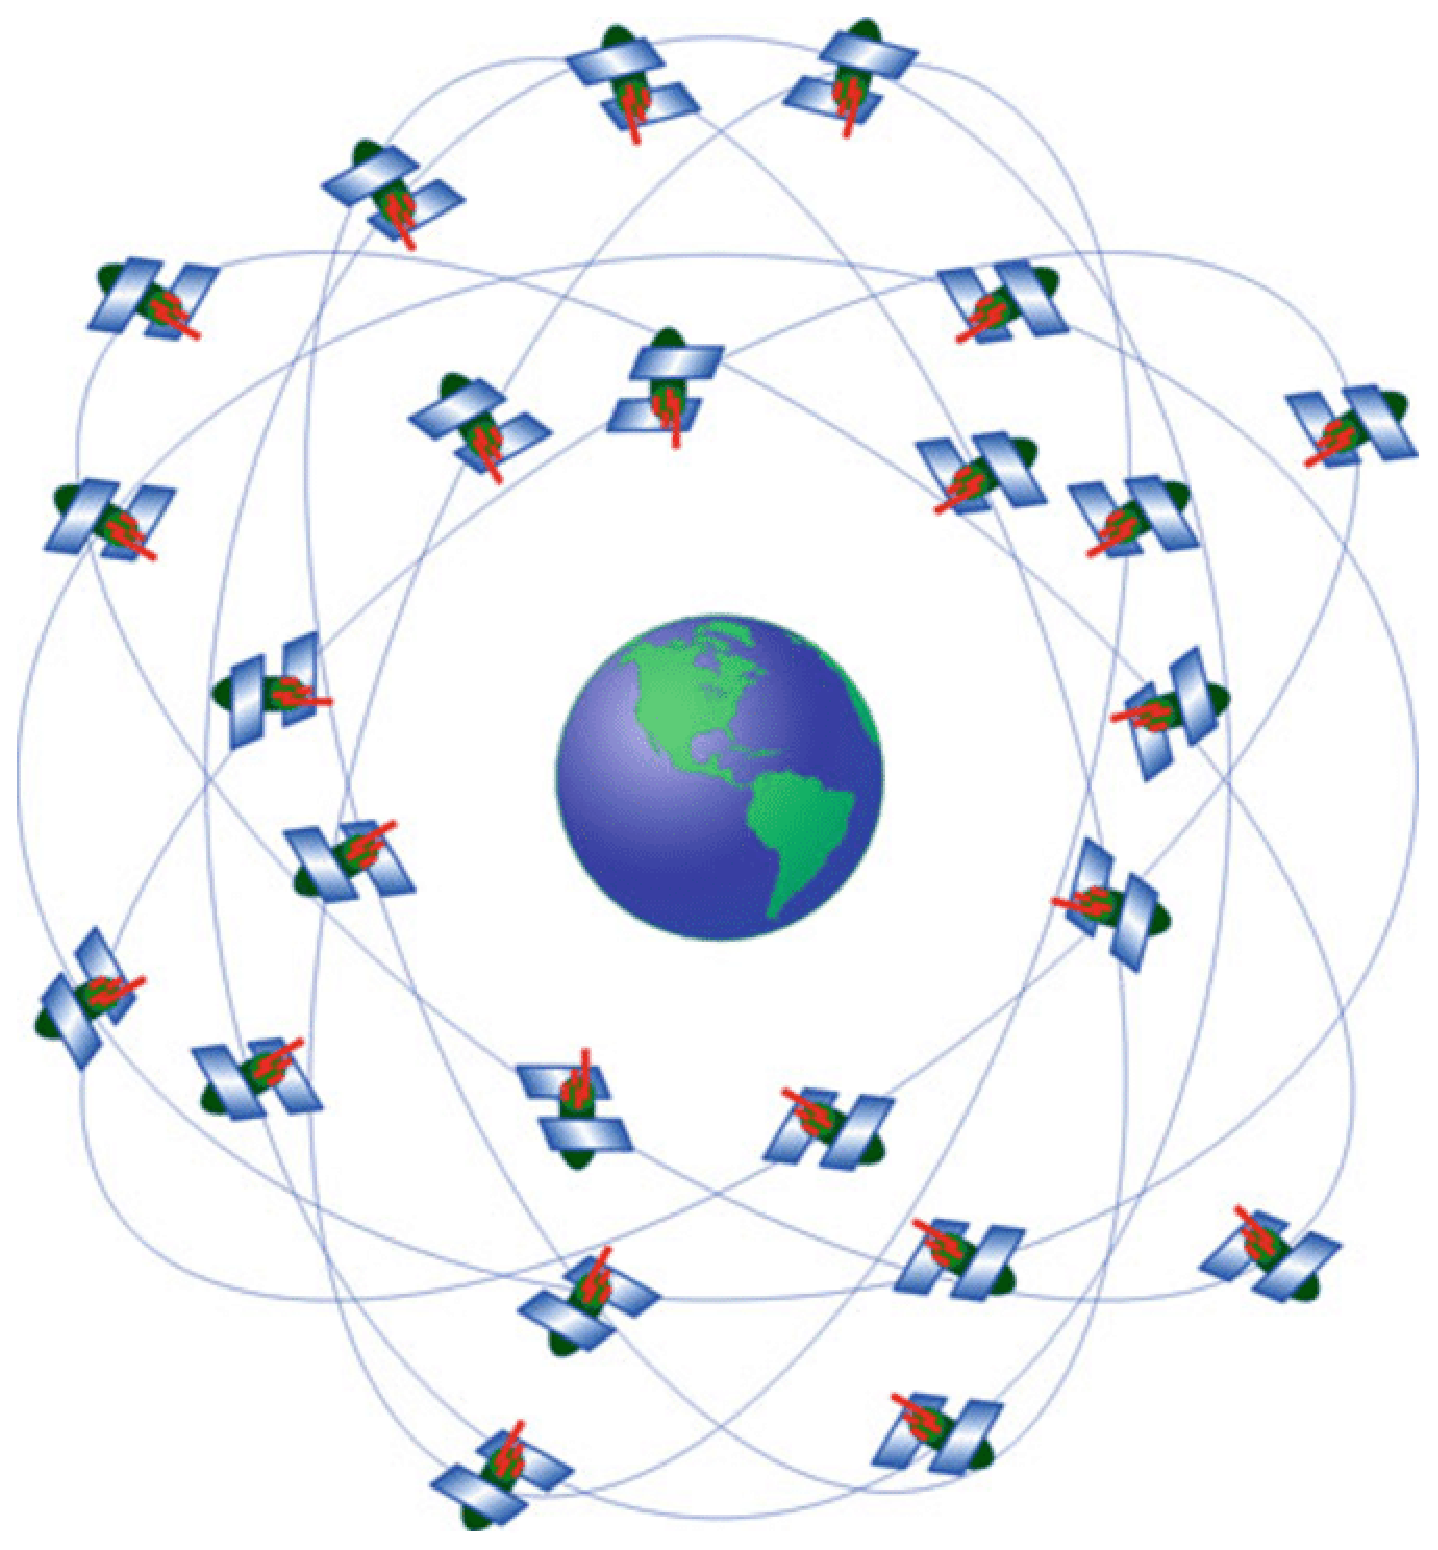
\includegraphics[width=4cm] {fig1-satellites.eps} \end{flushright}
\end{minipage}
\remarque{red}{!}{À mémoriser}
\cadre{
\begin{enumerate}
\item Pour pouvoir déterminer sa position sur Terre, son récepteur GPS doit pouvoir capter à tout moment   $\dots$ satellites

\item Les 3 coordonnées GPS sont définies par : 
\begin{itemize}
\item[$\bullet$] Le  méridien terrestre où on se situe donne la  \dotfill 
\item[$\bullet$] Le  parallèle  terrestre où on se situe  donne la \dotfill 
\item[$\bullet$] La  hauteur par rapport au niveau moyen de la mer donne l' \dotfill 
\end{itemize}
\end{enumerate}

}

\remarque{vert}{E}{Exercice}

Lancer un navigateur puis aller sur le site  \quad  \url{ https://www.coordonnees-gps.fr }

Déterminer alors les coordonnées GPS de la ville Saint-Romain-En-Gal 

\medskip

\begin{center}
Longitude :
\qquad \qquad\qquad Latitude :
\qquad\qquad\qquad  Altitude : 
\end{center}
\newpage

\begin{center}
{\large \textbf{Partie 2 : Conception d'un programme donnant la longitude et la latitude}}
\hrulefill
\end{center}


\remarque{orange}{>}{Principe}

Localement, on peut assimiler la sphère terrestre à un plan.

Ainsi, les coordonnées cartésiennes $(x;y)$ sont à variations proportionnelles  à la  latitude et à  la longitude

\remarque{vert}{E}{Exercice}

\begin{enumerate}
\item \begin{enumerate}
\item Lancer le programme Thonny.
\item Ouvrir le script \textit{ localisationGPS.py }  et l'exécuter.
\begin{center}
\includegraphics[width=9cm] {fig2-capture_ecran}
\end{center}

\item  À  l'aide du site  \url{ https://www.coordonnees-gps.fr }, remplir de tableau suivant :



\bigskip
\renewcommand{\arraystretch}{2}
\begin{tabular}{|c|c|c|c|c|c|c|}
\hline 
Ville & Saint-Romain en Gal & Paris & Marseille & Brest &Ajaccio &Toulouse\\ 
\hline 
abscisse (écran) : $x=$ & \qquad\qquad\qquad   &\qquad\qquad\qquad  & \qquad\qquad\qquad  & \qquad\qquad\qquad & \qquad\qquad\qquad & \qquad\qquad\qquad  \\ 
\hline 
ordonnée (écran): $y=$ &&&&&&  \\ 
\hline 
longitude :  &&&&&& \\ 
\hline 
latitude :  & & & &&&  \\ 
\hline 
\end{tabular} 

\end{enumerate}

\bigskip
\item La fonction $f$ permettant de passer de $x$ à la longitude est une fonction affine définie par $f(x)=ax+b$


\begin{minipage}[]{.4\textwidth}
\renewcommand{\arraystretch}{3}
\begin{tabular}{|c|c|c|c|}
\hline 
 &Ville& Paris & Marseille  \\
\hline 
 abscisse &$x$ &&   \\
\hline 
longitude &$f(x)$ && \\ 
\hline 
\end{tabular} 
\end{minipage}
\begin{minipage}[]{.6\textwidth}
\begin{enumerate}
\item 
À l'aide des données recueillies, écrire  un système d'équations,  d'inconnues  $a$ et $b$
\bigskip 
\bigskip 
\bigskip 
\bigskip 
\bigskip 
\bigskip 

\item À l'aide de la calculatrice Numworks, résoudre ce système.


Donner des arrondis des  valeurs de $a$ et $b$ obtenues :

\bigskip \bigskip 
\qquad \qquad $a= \dots $ \qquad \qquad \qquad \qquad \qquad $b=\dots$
\end{enumerate}
\end{minipage}

\newpage

\item De même, la fonction $g$ permettant de passer de $y$ à la lattitude est une fonction affine définie par $g(y)=my+p$


\begin{minipage}[]{.4\textwidth}
\renewcommand{\arraystretch}{3}
\begin{tabular}{|c|c|c|c|}
\hline 
 &Ville& Paris & Marseille  \\
\hline 
 ordonnée &$y$ &&   \\
\hline 
latitude &$g(y)$ && \\ 
\hline 
\end{tabular} 
\end{minipage}
\begin{minipage}[]{.6\textwidth}
\begin{enumerate}
\item 
À l'aide des données recueillies, écrire  un système d'équations,  d'inconnues  $m$ et $p$
\bigskip 
\bigskip 
\bigskip 
\bigskip 
\bigskip 
\bigskip 

\item À l'aide de la calculatrice Numworks, résoudre ce système.


Donner des arrondis des  valeurs de $m$ et $p$ obtenues :

\bigskip \bigskip 
\qquad \qquad $m= \dots $ \qquad \qquad \qquad \qquad \qquad $p=\dots$
\end{enumerate}
\end{minipage}

\bigskip \bigskip \bigskip \bigskip 
\item Résumé à compléter : 
\cadre{Formules permettant de calculer la longitude et la latitude en fonction des coordonnées $(x;y)$ sur l'écran :

\bigskip \bigskip 
Latitude : $g(y)=$


\bigskip \bigskip 
Longitude  : $f(x)= $



\bigskip\bigskip\bigskip
}


\item Traduction des formules précédentes en Python.


\begin{enumerate}
\item Ouvrir le script  l\textit{ocalisationGPSamelioration.py}
\item Compléter les lignes 37 et 44 selon les formules déterminée ci-dessous.


\begin{lstlisting}[numbers=left,firstnumber=35]
def g(y):
     	
     latitude =   
     
	
     return (int(latitude * 1000) / 1000.)

def f(x):
     	
     longitude =  
     
	
     return (int(longitude * 1000) / 1000.)

\end{lstlisting}

\item Enlever les dièses  des lignes 64 et 65 afin de les rendre exécutables.
\begin{lstlisting}[numbers=left,firstnumber=64]
canevas.create_text(850,300, text="longitude="+ str(f(x)),fill='red')  
canevas.create_text(850,330, text="latitude="+ str(g(y)),fill='blue')   
\end{lstlisting}   
\item Exécuter le script et vérifier que les affichages sont compatibles avec le tableau des 6 villes précédentes

\end{enumerate}
    
\end{enumerate}
\end{document}